\section {INOVAÇÃO SOCIAL ABERTA}
\label{inovacaosocialaberta}

A ideia de Inovação Social Aberta, surge da necessidade de fechar a lacuna das pesquisas de inovação aberta, que na grande maioria das vezes são focadas estritamente no setor privado. \cite{chesbrough2014}.

Como mostrado na sessão anterior de Inovação Social, \citeauthor{chesbrough2014} (\citeyear{chesbrough2014}, p. 201) trazem a mesma concepção de Inovação Social, e propõe que a Inovação Aberta contribua nas 6 etapas do modelo de Inovação Social proposto por \citeauthor{murray2010} (\citeyear{murray2010}), criando assim um novo conceito, o da Inovação Social Aberta. 

A Inovação Social Aberta é uma forma de realizar inovações voltadas para as necessidades existentes no meio social, tanto de dentro para fora quanto de fora para dentro. 

Segundo \citeauthor{chesbrough2014} (\citeyear{chesbrough2014}, p.202),
o processo de Inovação Social, através da sua "abertura", pode ser potencializado em suas seguintes etapas: prototipagem, sustentação dos esforços inovativos e escalonamento das soluções.
\par\vspace{1\baselineskip}

Segundo \citeauthor{gegenhuber2023} (\citeyear{gegenhuber2023}), a Inovação Social Aberta possui duas versões:
\begin{itemize}
    \item \textbf{Primeira versão (1.0):} inovação Social Aberta centrada na organização
    \item \textbf{Segunda versão (2.0):} inovação Social Aberta multissetorial, que  destaca  atividades  conjuntas  de  múltiplas  partes  interessadas  de  vários  setores  como  essenciais  para  abordar  problemas  sociais.
\end{itemize} 

\subsection{Inovação Social Aberta voltada para ONGs}

\citeauthor{gama2023} (\citeyear{gama2023}, p. 4) traz uma proposta de processo de Inovação Social Aberta baseado nos modelos de \citeauthor{chesbrough2014} (\citeyear{chesbrough2014}) e \citeauthor{murray2010} (\citeyear{murray2010}), porém, sem avançar a sexta etapa, que demandaria um tempo grande, sendo inviável para o trabalho. 

O campo da pesquisa foi uma,\gls{ONG}, que  auxilia  pessoas socialmente vulneráveis  que  vivem  com  HIV/AIDS, por meio de um \textit{hackathon} interdisciplinar com pessoas de três áreas do conhecimento (Psicologia, Design e Ciência da Computação), com o desenvolvimento de uma plataforma de \textit{software} funcional durante o período de 6 (seis) meses.

Esse modelo, segundo o autor, surgiu da necessidade de que boa parte dos processos de Inovação Social Aberta direcionado para \gls{ONG}s não conseguiam avançar da terceira etapa do modelo proposto por \citeauthor{murray2010} (\citeyear{murray2010}), a etapa de Prototipagem e pilotos. O processo proposto por \citeauthor{gama2023} (\citeyear{gama2023}) é divido em três fases:

\begin{figure}[H]
    \caption{Processo de Inovação Social Aberta para \gls{ONG}}
    \centering
    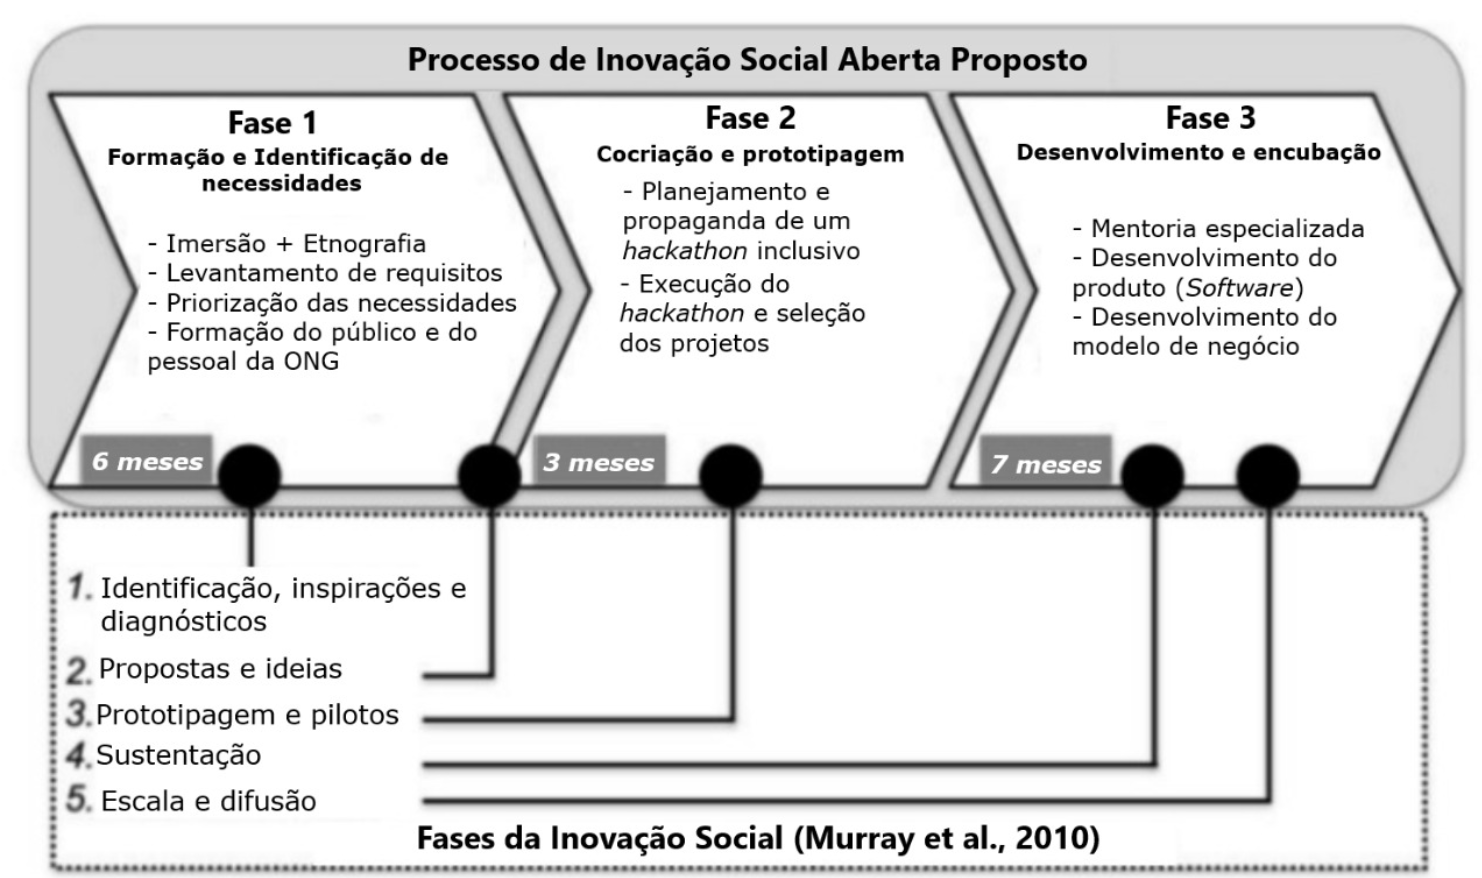
\includegraphics[width=\linewidth]{images/fundamentacao/isaong.png}
    \label{fig:isaong}
    
    Fonte: Adaptado de \citeauthor{gama2023} (\citeyear{gama2023}).
\end{figure}

\begin{itemize}
    \item \textbf{Fase 1 - Formação e identificação de necessidades:} possui um foco na etnografia, visando compreender o contexto e as necessidades dos usuários da organização, visando a identificação e validação das áreas que serão abordadas no processo de inovação. Também busca nivelar o conhecimento acerca de inovação para todos os participantes.
    \item \textbf{Fase 2 - Cocriação e prototipagem:} consiste na estruturação e planejamento do que será realizado, nesse caso, um \textit{hackathon}, além da divulgação para atrair participantes para a atividade proposta. Nessa fase também é realizado o levantamento dos requisitos dos usuários.
    \item \textbf{Fase 3 - Desenvolvimento e encubação:} essa fase é focada no desenvolvimento da solução proposta e incubação, pensando na sustentabilidade, escalabilidade e difusão dessa solução, nesse caso, baseada em software. O processo de desenvolvimento também engloba validação com a ONG, a fim de garantir que os requisitos levantados na fase anterior estão sendo atendidos.
\end{itemize}

